\slajdid{08-s023}
\begin{frame}[label=08-s023]
\gusttekst
Izlaz neopterećenog logičkog kola dat je funkcijom prenosa, odnosno prenosnom karakteristikom
\[V_o=f(V_i)\]
i predstavlja ulaz u neko naredno logičko kolo.\par\medskip
\centering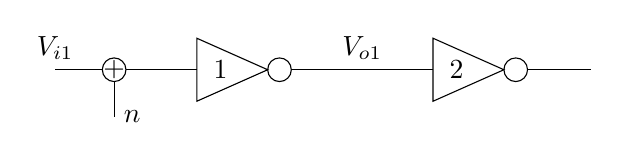
\begin{tikzpicture}[x=1cm,y=1cm,font=\sitneoznake]
\draw(-2.2,0)node[above]{$V_{i1}$}--(-1.6,0);\draw(-1.45,0)circle(.15)node{$+$};\draw(-1.45,-.6)node[right]{$n$}--(-1.45,-.15);\draw(-1.3,0)--(-.4,0);
\foreach\x/\num in{0/1,3/2}{\draw(\x-.4,.4)--(\x+.5,0)--(\x-.4,-.4)--cycle;\node at(\x-.1,0){\num};\draw(\x+.65,0)circle(.15);}
\draw(.8,0)--(2.6,0)node[midway,above]{$V_{o1}$};\draw(3.8,0)--(4.6,0);
\end{tikzpicture}

\[V_{O1}=f(V_{i1}+n)\]
\[V_{O1}=f(V_{i1}+n)=f(V_{i1})+n\frac{dV_o}{dV_i}+n^2\frac{d^2V_o}{dV_i^2}+\cdots\]
\bigskip
\[V_{O1}=f(V_{i1}+n)=f(V_{i1})+n\frac{dV_o}{dV_i}=f(V_{i1})+na\]
\end{frame}
